\label{sec:enquete-resultaten}

Onderstaande tabel bevat de resultaten van de enquête. In totaal zijn er 31 enquête-formulieren ingeleverd. Sommige vragen waren multiple choice en sommige op basis van een schaal naar belangrijkheid, waar 1 onbelangrijk is en 5 erg belangrijk.

\begin{figure}[ht]
  \begin{center}
    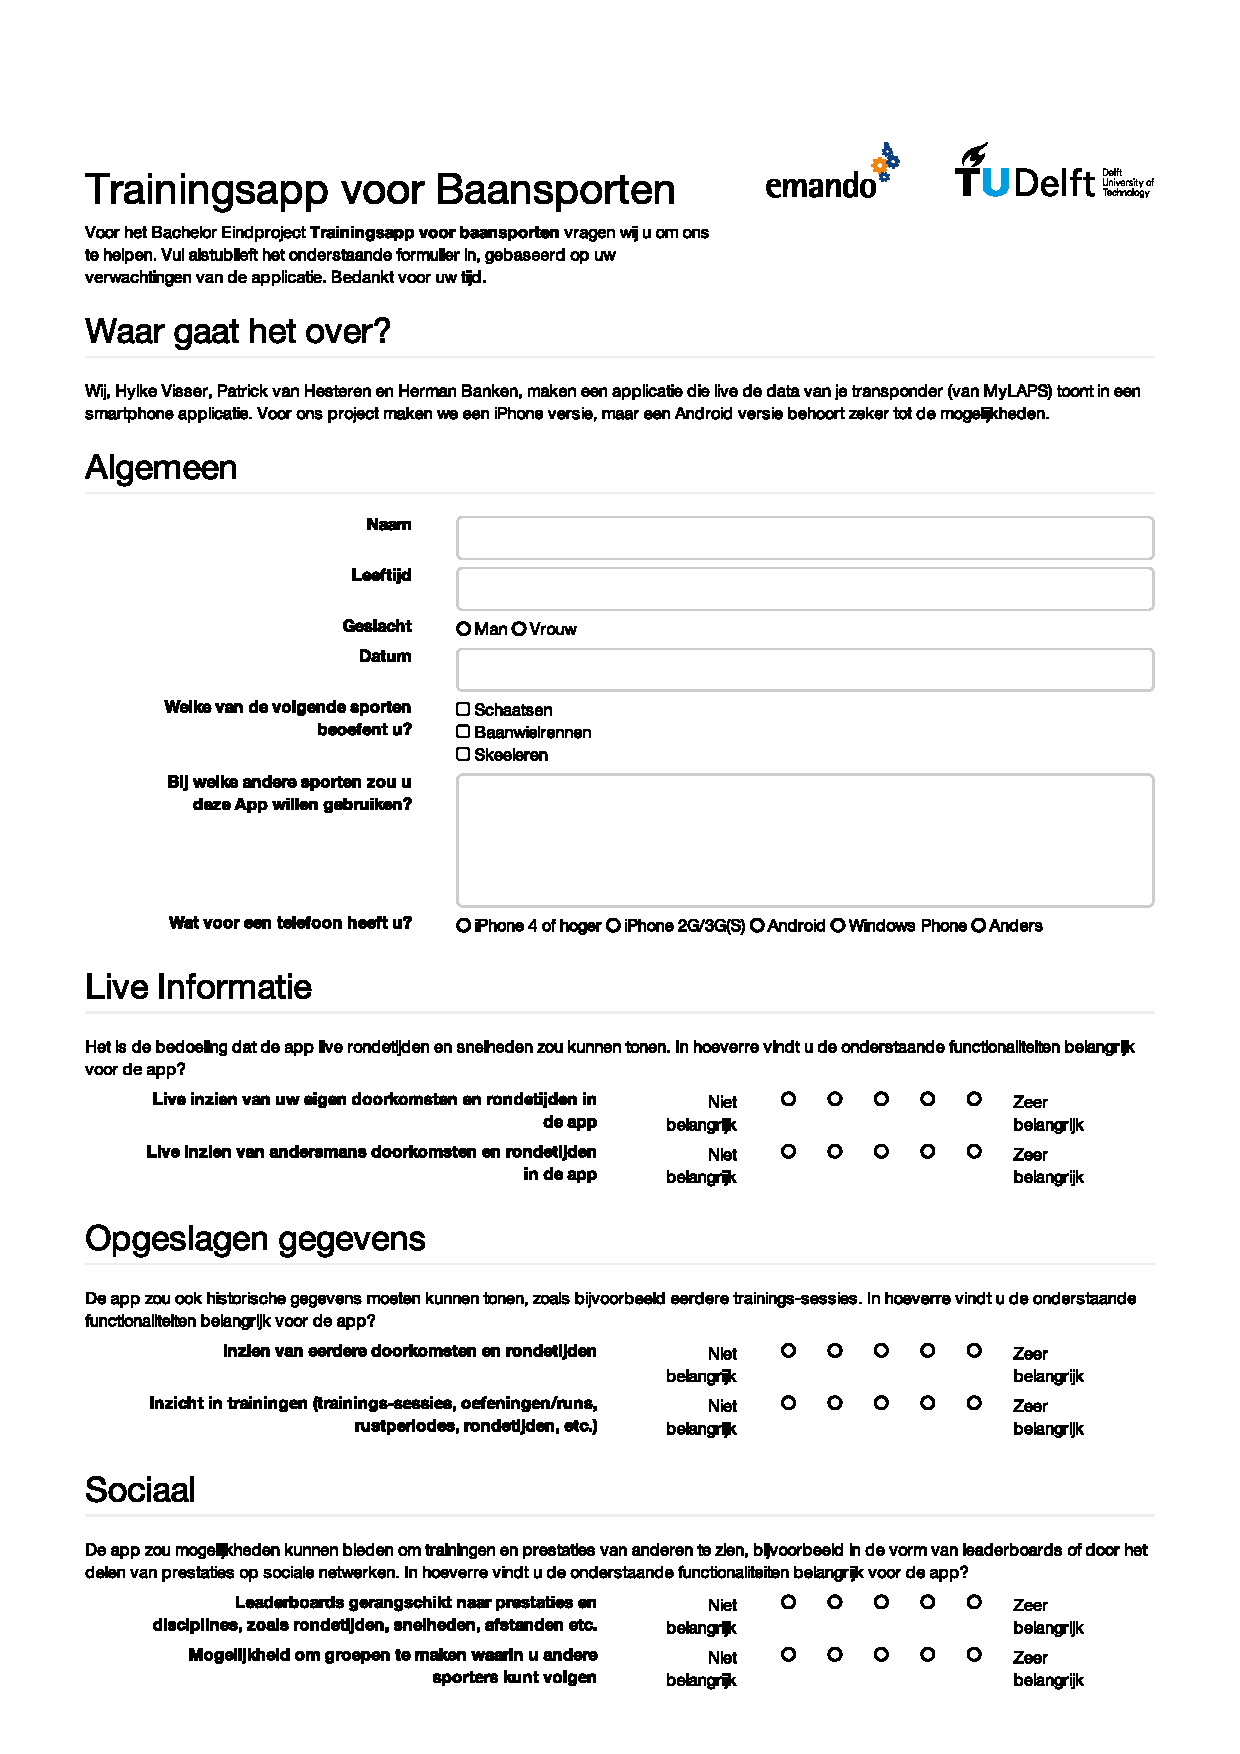
\includegraphics[width=\textwidth]{style/images/Enquete1}
  \end{center}
  \label{fig:enquete1}
\end{figure}

\begin{figure}[ht]
  \begin{center}
    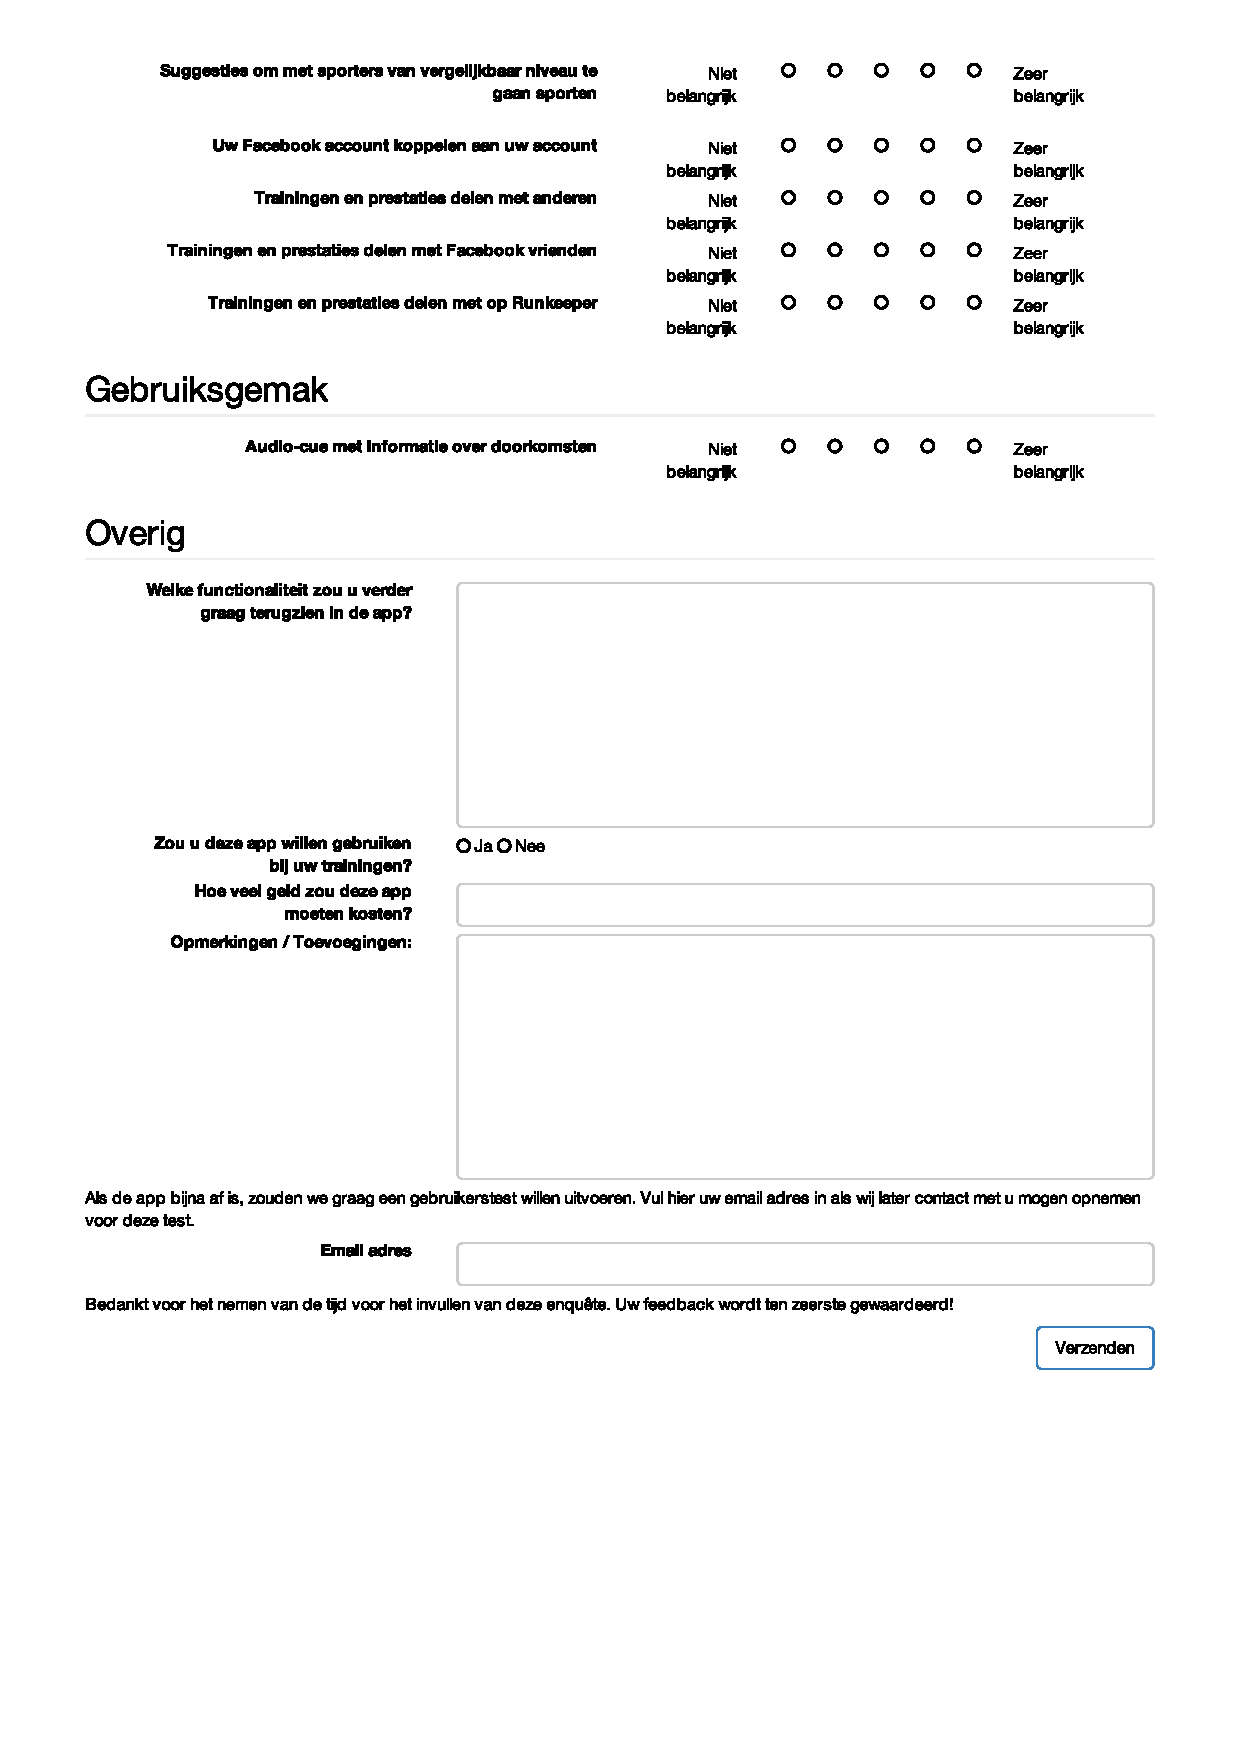
\includegraphics[width=\textwidth]{style/images/Enquete2}
  \end{center}
  \label{fig:enquete2}
\end{figure}

\begin{table}[h]
\begin{tabular}{| l | l | l |}
\hline
                         & \multicolumn{2}{l |}{Distributie of}                                                          \\ \hline
                         & Gemiddelde                                     & Standaard deviatie                           \\ \hline
\multicolumn{3}{l}{\textbf{Algemeen}}                                                                                  \\ \hline
Leeftijd                 & 24.1 jaar                                      & 9.0                                          \\ \hline
Geslacht                 & \multicolumn{2}{l|}{70\% man, 30\% vrouw}                                                     \\ \hline
Sporten                  & \multicolumn{2}{l|}{96.7\% Schaatsen, 66.7\% Skeeleren, 6,7\% Baanwielrennen}                 \\ \hline
Sporten overig           & \multicolumn{2}{l|}{Hardlopen, weg-wielrennen, athletiek}                                     \\ \hline
Telefoon                 & \multicolumn{2}{l|}{\begin{tabular}[c]{@{}l@{}}70.0\% Android, 23.3\% iPhone 4+\\ 3.3\% iPhone 2G/3G, 3.3\% Windows Phone\end{tabular}} \\ \hline
\multicolumn{3}{l}{\textbf{Live informatie}}                                                                           \\ \hline
Eigen doorkomsten        & 4.53 uit 5                                     & 0.73                                         \\ \hline
Andermans doorkomsten    & 3.47 uit 5                                     & 1.11                                         \\ \hline
\multicolumn{3}{l}{\textbf{Opgeslagen data}}                                                                           \\ \hline
Inzien doorkomsten       & 4.57 uit 5                                     & 0.63                                         \\ \hline
Inzicht in trainingen    & 4.30 uit 5                                     & 0.84                                         \\ \hline
\multicolumn{3}{l}{\textbf{Sociaal}}                                                                                   \\ \hline
Leaderboards             & 3.23 uit 5                                     & 0.94                                         \\ \hline
Groepen maken            & 3.83 uit 5                                     & 0.91                                         \\ \hline
Suggesties               & 2.73 uit 5                                     & 1.14                                         \\ \hline
Facebook login           & 2.13 uit 5                                     & 1.20                                         \\ \hline
Delen resultaten         & 2.67 uit 5                                     & 1.24                                         \\ \hline
Delen via FB             & 2.00 uit 5                                     & 1.20                                         \\ \hline
Delen via RunKeeper      & 1.63 uit 5                                     & 1.00                                         \\ \hline
\multicolumn{3}{l}{\textbf{Gebruiksgemak}}                                                                             \\ \hline
Audio-cue                & 3.83 uit 5                                     & 1.26                                         \\ \hline
\multicolumn{3}{l}{\textbf{Overig}}                                                                                    \\ \hline
De app willen gebruiken  & \multicolumn{2}{l|}{96.7\% ja, 3.3\% nee}                                                     \\ \hline
Wat de app mag kosten    & € 1.72                                         & 2.13                                         \\ \hline               
\end{tabular}
\end{table}

\newpage

\section*{Verdere functionaliteit opgegeven door respondenten}
\begin{itemize}
\item Tijdsverschillen tussen de rondjes (mobiel bij trainer en rondetijden gelijk terugkijken na oefening)
\item Actuele snelheid zou wel vet zijn. Of een verwachte rondetijd op basis van de huidige snelheid.
\item Trainingen en prestaties delen met endomondo
\item Hardslagmeter, calorieën-schatter. Suggesties voor trainingschema's: lange termijn (intensievere trainingsweek of extensievere trainingsweek) en korte termijn (schaats-schema's die te laden zijn en aan de prestatie gekoppeld worden).
\item Gebruiksvriendelijk, snelheid bv: snel opgestart, etc. De Hockey-WK-app is bijvoorbeeld erg traag en dat is echt niet fijn.
\item Vooraf ingesteld trainingsschema (wat nu gaan doen?) \item Tussentijdse feedback op rijden (tijdens het rijden een piep voor elke "100" meter (niet echt honderd meter, maar herkenbare punten: ingaan bocht/rechte eind, passeren van 1000m start, enz als je een bepaald tempo moet rijden bijvoorbeeld.
\item Tijdens training liever niet vergelijken met anderem, achteraf wel leuk.
\item Misschien een mogelijkheid om je trainingsschema vooraf in te vullen. Dan kun je vervolgens live zien of je dat ook aan het bewerkstelligen bent of dat je niet doet wat je moest doen. Chearleaders die je aanmoedigen als je een beetje achterop raakt op je schema en het boze hoofd van John de Wolf als je gefaald hebt zijn bonus.
\item Metingen op basis van gps en niet alleen via transponders (als dat mogelijk is, vooral handig voor skeeleren).
\item Misschien een rondeteller (zoals die oude mannetjes altijd hebben) voor als je veel rondjes gaat rijden en het zou ook wel vet zijn als je ook je hartslag erbij kan zien, maar dat is voor de echte pro's!
\end{itemize}

\section*{Overige opmerkingen door respondenten}

\begin{itemize}
\item Leuk bedacht, alleen jammer dat je er een transponder voor nodig hebt, wordt het gelijk wel duur. Zou dit ook met GPS kunnen?
\item Het zou wel geniaal zijn als je via je oortjes je hele trainingsschema te horen krijgt en deze vervolgens rijdt en dat de app weet hoe ver je steeds bent. En het lijkt me een vooruitgang dat je real-time weet hoe je snel je de afstanden aflegt, zodat je bijvoorbeeld een vlak of oplopend schema kan rijden.
\item Altijd met telefoon in de hand wordt de ijsbaan niet veiliger van. Denk goed na wanneer je je tel wel/niet in de hand hebt.
\item Een van de belangrijkste punten is wat mij betreft de audiofeedback tijdens het sporten. Het terugkijken van gereden tijden is leuk, maar direct feedback tijdens het sporten werkt voor mij (uit ervaring met RunTastic apps voor hardlopen en wielrennen) erg motiverend.
\item iPhone 4 en verder zijn in dit onderzoek onder een noemer gebracht. Ik merk nu al dat de RunTastic apps, die inmiddels geoptimaliseerd zijn voor iPhone 5C/S, behoorlijk trager werken op iPhone 4. Het zou geweldig zijn als deze app ook soepel runt op iPhone 4. 
\item Werkt de app ook zonder transponder, bijvoorbeeld op GPS?
\end{itemize}